\documentclass[10pt]{article}

\usepackage[margin=1in]{geometry}
\setlength{\tabcolsep}{18pt}
\renewcommand{\arraystretch}{1.5}
\usepackage[table]{xcolor}
\usepackage{fontspec} 
\usepackage{graphicx}
\usepackage{listings}
\usepackage{xcolor}
\usepackage{wrapfig}
\definecolor{codegreen}{rgb}{0,0.6,0}
\definecolor{codegray}{rgb}{0.5,0.5,0.5}
\definecolor{codepurple}{rgb}{0.58,0,0.82}
\definecolor{backcolour}{rgb}{0.95,0.95,0.92}
\lstdefinestyle{mystyle}{
	backgroundcolor=\color{backcolour},   
	commentstyle=\color{codegreen},
	keywordstyle=\color{magenta},
	numberstyle=\tiny\color{codegray},
	stringstyle=\color{codepurple},
	basicstyle=\ttfamily\footnotesize,
	breakatwhitespace=false,         
	breaklines=true,                 
	captionpos=b,                     
	numbers=left,                    
	numbersep=5pt,                  
	showspaces=false,                
	showstringspaces=false,
	showtabs=false,
}
\lstset{style=mystyle}
\setmainfont{Arial}
\graphicspath{ {./} }

\begin{document}
	
	\begin{titlepage} % Suppresses displaying the page number on the title page and the subsequent page counts as page 1
		\newcommand{\HRule}{\rule{\linewidth}{0.5mm}} % Defines a new command for horizontal lines, change thickness here
		
		\center % Centre everything on the page
		
		%------------------------------------------------
		%	Headings
		%------------------------------------------------
		
		\textsc{\LARGE Universita' degli studi di Padova}\\[1.5cm] % Main heading such as the name of your university/college
		
		\textsc{\Large D4C Cinemas}\\[0.5cm] % Major heading such as course name
		
		
		%------------------------------------------------
		%	Title
		%------------------------------------------------
		
		\HRule\\[0.4cm]
		
		{\huge\bfseries Progetto Basi di Dati}\\[0.2cm] % Title of your document
		
		\HRule\\[1.5cm]
		
		%------------------------------------------------
		%	Author(s)
		%------------------------------------------------
		
		\begin{minipage}{0.4\textwidth}
			\begin{flushleft}
				\large
				Damiano \textsc{Bertoldo} % Your name
			\end{flushleft}
		\end{minipage}
		~
		\begin{minipage}{0.4\textwidth}
			\begin{flushright}
				\large
				Alessandro \textsc{Canel} % Supervisor's name
			\end{flushright}
		\end{minipage}
		
		% If you don't want a supervisor, uncomment the two lines below and comment the code above
		{\large\textit{}}\\
		\textsc{2019/2020} % Your name
		
		%------------------------------------------------
		%	Date
		%------------------------------------------------
		
		\vfill\vfill\vfill % Position the date 3/4 down the remaining page
		
		
		%------------------------------------------------
		%	Logo
		%------------------------------------------------
		
		%\vfill\vfill
		%\includegraphics[width=0.2\textwidth]{placeholder.jpg}\\[1cm] % Include a department/university logo - this will require the graphicx package
		
		%----------------------------------------------------------------------------------------
		
		\vfill % Push the date up 1/4 of the remaining page		
		\tableofcontents
	\end{titlepage}
	\section{Abstract}	
	La societa' D4C Cinemas e' una catena di cinema, nata in regno unito nel 1988 da una partnership tra Universal Studios e Paramount Pictures che nel corso degli anni si e' estesa sia nel campo nazionale, che nel campo internazionale. \\
	Si vuole gestire la base di dati del cinema, comprendente la gestione di piu' cinema contemporaneamente. Ogni cinema e' un multisala contenente dalle 5 alle 10 sale ed ogni sala ha dai 50 ai 250 posti. D4C Cinemas rilascia giornalmente la programmazione degli spettacoli in modo tale da dare ai clienti varia scelta per l'orario che desiderano. Una persona per acquistare un biglietto deve recarsi alla biglietteria e al momento dell'acquisto comunicare le credenziali, dato che il biglietto e' nominativo a differenza di altri cinema. Ogni biglietto ha un prezzo fisso di 10 euro. Altra caratteristica di questa catena e' che al momento dell'uscita dalla sala lo spettatore puo' lasciare una recensione a caldo del film appena visto, cosi' da lasciare ai futuri spettatori la propria opinione. Altra cosa che viene effettuata in questa catena e' l'aggiunta e il tracciamento dei cast presenti, in modo tale da dare al cliente la possibilita' di avere la lista di film in cui recita il proprio attore/regista/sceneggiatore/produttore preferito.
	\section{Analisi dei requisiti}
	
	Il progetto vuole rappresentare una base di dati che permetta di gestire la programmazione dei film della catena D4C cinema.
			
	Essendo D4C cinemas una catena, e' necessario identificare ciascun {\bf Cinema}:
	\begin{itemize}
		\item Nome cinema
		\item Indirizzo, cosi' composto: via, citta', numero civico, codice postale, nazione
	\end{itemize}
	Per poter identificare una {\bf Sala} all'interno del cinema abbiamo bisogno delle sguenti informazioni:
	\begin{itemize}
		\item Numero sala (univoco all'interno del cinema)
		\item Cinema di appartenenza
		\item Numero posti
		\item Grandezza schermo (espresso in pollici)
	\end{itemize}
	Per ogni Sala vengono proiettati vari film durante la giornata. Tali orari sono definiti nell'entita' {\bf Spettacolo}:
	\begin{itemize}
		\item Film
		\item Sala di proiezione
	    \item Data ora film
	    \item 3D
	    \item Posti venduti
	\end{itemize}
	I clienti del cinema durante la scelta del film devono avere la possibilita' di consultare le informazioni dei vari \textbf{Film}, dati necessari anche per l'organizzazione degli spettacoli:
	\begin{itemize}
		\item Titolo
		\item Durata
		\item Trama
		\item Genere
		\item Anno
	\end{itemize}
	Ciascun film è prodotto da un cast {\bf Cast}, di cui si conosce:
	\begin{itemize}
		\item Nome
	\end{itemize}
	Per sapere da chi e' composto il cast del film, e' necesssario avere nome e ruolo delle persone che ne hanno fatto parte, dette persone fanno parte dell'entità {\bf Lavoratore}, e viene inteso come persone che hanno lavorato con mansioni in ambito cinematografico:
	\begin{itemize}
		\item Persona
		\item Cast
		\item Salario
	\end{itemize}
	Lavoratore a sua volta ha come sottocategoria le seguenti mansioni, dato che lavoratore viene inteso come persona che ha partecipato in mansioni per la relizzazione di un film:
	\begin{itemize}
		\item {\bf Attore}: persona che ha recitato nel film 
		\item {\bf Sceneggiatore}: persona che ha strutturato la sceneggiatura del film 
		\item {\bf Produttore}: persona che ha finanziato il film 
		\item {\bf Regista}: persona che ha diretto il film
	\end{itemize}		 
	Di conseguenza è necessario definire {\bf Persona}, in quanto ogni {\bf Lavoratore} è per l'appunto, una persona e quindi tale entità dovra comprendere:
	\begin{itemize}
		\item Nome
		\item Cognome
		\item Data di nascita
		\item Sesso
	\end{itemize}
	Ogni persona in quanto tale, potrà acquistare un biglietto per un qualsivoglia film. Il {\bf Biglietto} conterrà:
	\begin{itemize}
		\item Persona di appartenenza
		\item Spettacolo
		\item Numero posto
	\end{itemize}
	Qualsiasi persona potrà inoltre rilasciare una {\bf Recensione} inerente al film appnea visto. L'entità recensione conterrà:
	\begin{itemize}
		\item Persona
		\item Film
		\item Commento
		\item Voto
	\end{itemize}
 	\subsection{Lista delle operazioni}		
	\textbf{Operazione 1}: Aggiuta di uno spettacolo per la proiezione di un film in una sala (40 volte al giorno) \\
	\textbf{Operazione 2}: Emissione biglietti (2500 volte al giorno)\\
	\textbf{Operazione 3}: Aggiunta nuovi film (5 volte al mese)\\
	\textbf{Operazione 4}: Rilascio di una recensione (2200 volte al giorno)\\
	\textbf{Operazione 5}: Aggiunta di un nuovo cast (4 volte al mese)\\
	\textbf{Operazione 6}: Conteggio totale posti venduti per ogni spettacolo (1 volta a settimana)
 	\subsection{Glossario dei termini}
 	\begin{tabular}{ |p{3cm}|p{4.5cm}|p{2.5cm}|p{3cm}|  }
 		%\hline
 		%\multicolumn{4}{|c|}{\textbf{Glossario dei termini}} \\
 		\hline
 		\rowcolor{lightgray}
 		\textbf{Termine} & \textbf{Descrizione} & \textbf{Sinonimi} & \textbf{Collegamenti} \\
 		\hline
 		Spettacolo                         & Manifestazione artistica o ricreativa presentata a un pubblico               &                                                                                      & Biglietto, Film, Sala                                                             \\ \hline
 		Sala                                   & Stanza dove viene proiettato il Film                                    &                                                                                      & Cinema, Spettacolo \\ \hline
 		Biglietto                              & Acquisto del cliente, che attesta la vendita del posto per un dato film &                                                                                      & Spettacolo, Persona                                                               \\ \hline
 		Lavoratore                                & Persona che lavora all'interno di un cast             & Attore, Sceneggiatore, Produttore, Regista & Cast, Persona                                                                        \\ \hline
 		Cast & Gruppo di lavoratori che ha preso parte alla realizzazione del film &  & Lavoratore,Film \\ \hline 
 		
 		Persona & Persona cliente del cinema e/o lavoratore & & Recesione, Biglietto
 		        \\ \hline
 		Film                                   & Film presenti al cinema                                                 &                                                                                      & Cast, Recensione, Spettacolo       \\ \hline
 		Cinema                                   &    Impresa che offre il servizio cinematografico &                                                                                      &  Sala        \\ \hline
 		Recensione                               & Recensioni da clienti paganti
 		&                                       & Film, Persona \\ \hline
 	\end{tabular}
 	\subsection{Strutturazione dei requisiti}
	\begin{tabular} { |p{16.8cm}| }
 		\hline
 		\rowcolor{lightgray}
 		\textbf{Frasi relative a "Cinema"} \\
 		\hline
 		I Cinema vengono identificati tramite: Nome cinema, Indirizzo (composto da via, citta', numero civico, codice postale, nazione) \\
 		\hline 		
 	\end{tabular}
 	\\\\\\
	\begin{tabular} { |p{16.8cm}| }
	 	\hline
	 	\rowcolor{lightgray}
	 	\textbf{Frasi relative a "Sala"} \\
	 	\hline
	 	Le Sale vengono identificate tramite: Numero sala (univoco all'interno del cinema), Cinema di appartenenza, Numero posti, Grandezza schermo (espresso in pollici) \\
	 	\hline 		
	\end{tabular} 
	\\\\\\
	\begin{tabular} { |p{16.8cm}| }
		\hline
		\rowcolor{lightgray}
		\textbf{Frasi relative a "Spettacolo"} \\
		\hline
		Lo spettacolo viene idetificato tramite: Data e ora inizio spettacolo, Se il film è 3D o no, posti venduti \\
		\hline 		
	\end{tabular} 
	\\\\\\
	\begin{tabular} { |p{16.8cm}| }
		\hline
		\rowcolor{lightgray}
		\textbf{Frasi relative a "Film"} \\
		\hline
		I Film vengono identificati tramite: Titolo, Durata, Trama, Genere, Anno \\
		\hline 		
	\end{tabular} 
 	\\\\\\
 	\begin{tabular} { |p{16.8cm}| }
 		\hline
 		\rowcolor{lightgray}
 		\textbf{Frasi relative a "Cast"} \\
 		\hline
 		Il Cast viene identificato tramite: Nome \\
 		\hline 		
 	\end{tabular} 
 	\\\\\\
 	\begin{tabular} { |p{16.8cm}| }
 		\hline
 		\rowcolor{lightgray}
 		\textbf{Frasi relative a "Lavoratore"} \\
 		\hline
 		I Lavoratori vengono identificati tramite: Persona, Cast, Salario \\
 		\hline 		
 	\end{tabular} 
 	\\\\\\
 	\begin{tabular} { |p{16.8cm}| }
 		\hline
 		\rowcolor{lightgray}
 		\textbf{Frasi relative a "Persona"} \\
 		\hline
 		Le Persone vengono identificate tramite: Nome, Cognome, Data nascita e Sesso \\
 		\hline 		
 	\end{tabular} 
 	\\\\\\
 	\begin{tabular} { |p{16.8cm}| }
 		\hline
 		\rowcolor{lightgray}
 		\textbf{Frasi relative a "Recensione"} \\
 		\hline
 		Le recensioni vengono identificati tramite: Persona, Film, Commento, Voto \\
 		\hline 		
 	\end{tabular} 
 	\\\\\\
 	\begin{tabular} { |p{16.8cm}| }
 		\hline
 		\rowcolor{lightgray}
 		\textbf{Frasi relative a "Attore"} \\
 		\hline
 		Lavoratore che ha lavorato come attore nel film \\
 		\hline 		
 	\end{tabular} 
	\\\\\\
	\begin{tabular} { |p{16.8cm}| }
		\hline
		\rowcolor{lightgray}
		\textbf{Frasi relative a "Sceneggiatore"} \\
		\hline
		Lavoratore che ha lavorato come sceneggiatore nel film \\
		\hline 		
	\end{tabular} 
	\\\\\\
	\begin{tabular} { |p{16.8cm}| }
		\hline
		\rowcolor{lightgray}
		\textbf{Frasi relative a "Produttore"} \\
		\hline
		Lavoratore che ha lavorato come produttore nel film \\
		\hline 		
	\end{tabular} 
	\\\\\\
	\begin{tabular} { |p{16.8cm}| }
		\hline
		\rowcolor{lightgray}
		\textbf{Frasi relative a "Regista"} \\
		\hline
		Lavoratore che ha lavorato come regista nel film \\
		\hline 		
	\end{tabular} 
	\\\\\\
	\begin{tabular} { |p{16.8cm}| }
		\hline
		\rowcolor{lightgray}
		\textbf{Frasi relative a "Biglietto"} \\
		\hline
		I Biglietti vengono idetificati tramite: Numero posto \\
		\hline 		
	\end{tabular} 
	\\\\\\
	
	
	\section{Progettazione Concettuale}	
	\subsection{Lista delle entita'}
	Di seguito veranno riportate le classi che verranno contenute nel database, tutti i campi sono \textbf{not null} tranne quelli specificati.\\
	\begin{itemize}
		\item \textbf{Cinema}: Rappresenta un cinema.
		\begin{itemize}
			\item Nome: \textit{string} univoco
			\item Indirizzo: attributo composto
				\subitem Via: \textit{string}
				\subitem Citta': \textit{string}
				\subitem Provincia: \textit{string}
				\subitem CAP: \textit{int}
				\subitem Regione: \textit{string}
				\subitem Nazione: \textit{string}			
		\end{itemize}
		\item \textbf{Sala}: Rappresenta una sala di un cinema.
		\begin{itemize}
		    \item Numero: \textit{int}
		    \item Cinema: \textit{string}
			\item Capienza: \textit{int}
			\item Grandezza\_schermo: \textit{int}
		\end{itemize}
		\item \textbf{Spettacolo}: Rappresenta dati per la Programmazione.
		\begin{itemize}
			\item DataOra\_Inizio: \textit{timestamp}
			\item 3D: \textit{bool}
			\item Posti\_Venduti: \textit{int}
		\end{itemize}
		\item \textbf{Biglietto}: Rappresenta il biglietto venduto.
		\begin{itemize}
			\item N\_Posto: \textit{int}
		\end{itemize}
		\item \textbf{Film}: Rappresenta un film.
		\begin{itemize}
			\item Titolo: \textit{string}
			\item Anno: \textit{int}
			\item Durata: \textit{time}
			\item Genere: \textit{string}
			\item Trama: \textit{string}
		\end{itemize}
		\item \textbf{Cast}: Rappresenta il nome del cast.
		\begin{itemize}
			\item Nome: \textit{string}
		\end{itemize}
		\item \textbf{Lavoratore}: Rappresenta una persona partecipante nel cast.
		\begin{itemize}
			\item Salario: \textit{int}
		\end{itemize}
		\item \textbf{Attore}: Specializzazione di Lavoratore
		\begin{itemize}
			\item Nessun Attributo
		\end{itemize}
		\item \textbf{Produttore}: Specializzazione di Lavoratore
		\begin{itemize}
			\item Nessun Attributo
		\end{itemize}
		\item \textbf{Sceneggiatore}: Specializzazione di Lavoratore
		\begin{itemize}
			\item Nessun Attributo
		\end{itemize}
		\item \textbf{Regista}: Specializzazione di Lavoratore
		\begin{itemize}
			\item Nessun Attributo
		\end{itemize}
		\item \textbf{Persona}: Rappresenta una persona che acquista i biglietti e/o fà parte della produzione del film
		\begin{itemize}
			\item Nome: \textit{string}
			\item Cognome: \textit{string}
			\item Data\_di\_nascita: \textit{datetime}	
			\item Sesso: \textit{string}
		\end{itemize}
		\item \textbf{Recensione}: Rappresenta la recensione di un film da parte di una persona.
		\begin{itemize}
			\item Commento: \textit{string}, possibilita' di null se la persona non rilascia un commento
			\item Voto: \textit{int}
		\end{itemize}
	\end{itemize}
	\subsection{Lista delle associazioni}
	Tutte le entità sono legate nel seguente modo:
	\begin{itemize}
	    \item {\textbf{Cinema-Sala: \underline{Appartiene}}
		    \begin{itemize}
			    \item Ogni cinema può avere diverse sale
			    \item Ogni sala può appartenere solo ad un cinema
			    \item Associazione di tipo (1,N) uno a molti
		    \end{itemize}}
		    
		\item {\textbf{Sala-Spettacolo: \underline{Assegnata}}
		    \begin{itemize}
			    \item Ogni sala può aver assegnati diversi spettacoli
			    \item Ogni spettacolo e' proiettato in una sala
			    \item Associazione di tipo (1,N) uno a molti
		    \end{itemize}}
		        
		\item {\textbf{Spettacolo-Film: \underline{Assegnato}}
		    \begin{itemize}
			    \item Ogni Spettacolo riproduce un solo Film
			    \item Un film può essere utilizzato per diversi Spettacoli 
			    \item Associazione di tipo (1,N) uno a molti
		    \end{itemize}}
		    
		\item {\textbf{Film-Cast: \underline{Lavora}}
		    \begin{itemize}
			    \item Ogni Cast può Lavorare a molti Film
			    \item Un film può avere solo un cast 
			    \item Associazione di tipo (1,N) uno a molti
		    \end{itemize}}
		
		\item {\textbf{Cast-Lavoratore: \underline{Partecipa}}
		    \begin{itemize}
			    \item Ad un Cast partecipano diversi lavoratori
			    \item Un lavoratore e' assegnato ad un cast con uno specifico ruolo
			    \item Associazione di tipo (1,N) uno a molti
		    \end{itemize}}
		  
		\item {\textbf{Persona-Recensione: \underline{Rilascia}}
		    \begin{itemize}
			    \item Ogni Persona può scrivere diverse Recensioni 
			    \item Ogni Recensione e' scritta da una sola persona 
			    \item Associazione di tipo (1,N) uno a molti
		    \end{itemize}}  
		    
		\item {\textbf{Recensione-Film: \underline{Ottiene}}
		    \begin{itemize}
			    \item  Ogni Recensione riguarda un solo film
			    \item  Qualsivoglia Film può ricevere diverse recensioni da parte delle persone 			    
			    \item Associazione di tipo (1,N) uno a molti
		    \end{itemize}}  
		    
		\item {\textbf{Persona-Biglietto: \underline{Compra}}
		    \begin{itemize}
			    \item  Ogni persona può comprare biglietti per vari film
			    \item  Ogni biglietto è intestato ad una sola persona
			    \item Associazione di tipo (1,N) uno a molti
		    \end{itemize}}  
		
		\item {\textbf{Biglietto-Spettacolo: \underline{Fà riferimento}}
		    \begin{itemize}
			    \item  Un biglietto fà riferimento ad un solo spettacolo
			    \item  Per ogni spettacolo vengono comprati diversi biglietti
			    \item Associazione di tipo (1,N) uno a molti
		    \end{itemize}}		 
    \end{itemize}
	\subsection{Schema ER}	
	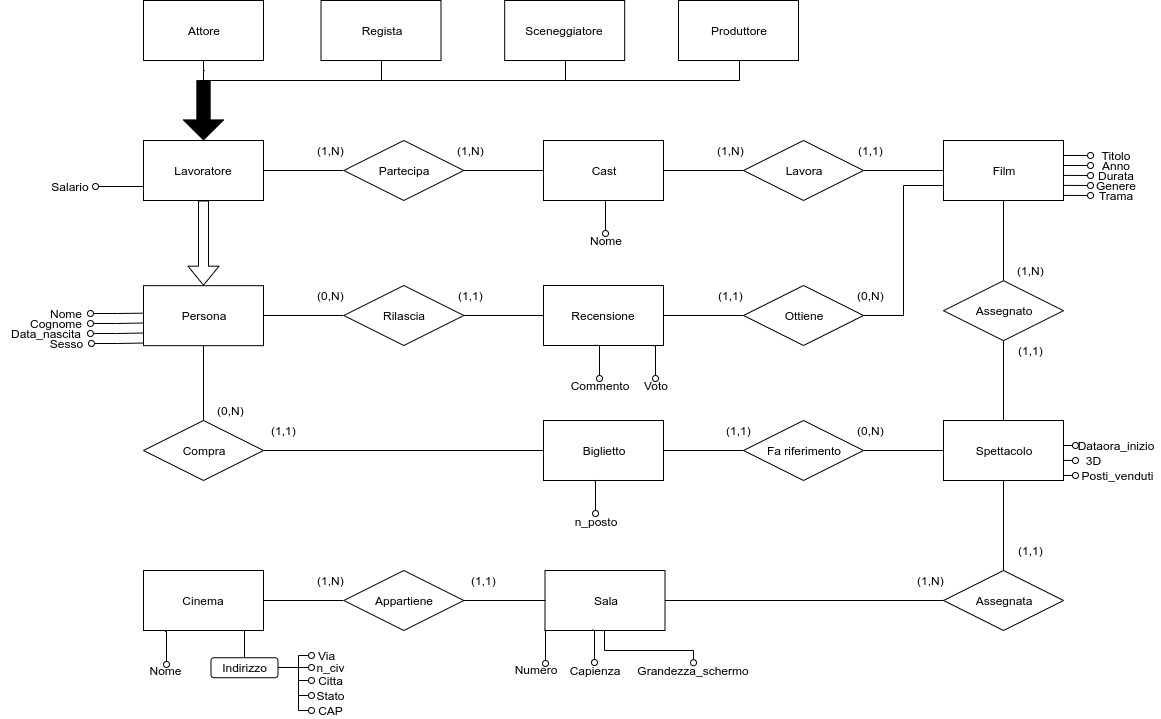
\includegraphics[width=\textwidth, height=16.1cm]{Schemas/SchemaER}
	\section{Progettazione logica}
	\subsection{Analisi ridondanza}	
	Una ridondanza si trova nell'entita' \textbf{Spettacolo}, nella quale l'attributo \textbf{posti\_venduti} si puo' calcolare visitando la relazione \textbf{Spettacolo-Biglietto} (chiamata "fa riferimento") e contando le occorrenze di tale relazione.
	\begin{table}[!h]
		\centering
		\begin{tabular}{|c|c|c|}
			\hline
			\textbf{Concetto} & \textbf{Tipo} & \textbf{Volume} \\
			\hline
			Spettacolo & E & 200 \\
			\hline
			Biglietto & E & 28000 \\
			\hline
			Fa' Riferimento & R & 28000 \\
			\hline
		\end{tabular}
	\end{table}
	\begin{itemize}
		\item \textbf{Operazione 2}: Emissione biglietti (2500 volte al giorno)
		\item \textbf{Operazione 6}: Conteggio totale posti venduti per ogni spettacolo (1 volta a settimana)		
	\end{itemize}
	L'operazione 6 ha come scopo contare l'affluenza settimanale dei clienti.\\
	Di seguito le operazioni di conteggio in scrittura verranno considerate doppie perche' operazioni piu onerose rispetto alle operazioni di lettura.
	\subsubsection{Presenza di ridondanza}
	L'attributo \textbf{posti\_venduti}, cosi' come indicato nello schema ER, indica il numero totale di posti venduti per uno spettacolo.
	\begin{table}[h!]
		\centering
		\caption{\textbf{Operazione 2 con ridondanza}} \label{tab:Op2 ridondanza}
		\begin{tabular}{|c|c|c|c|}
			\hline
			\textbf{Concetto} & \textbf{Costrutto} & \textbf{Accessi} & \textbf{Tipo} \\
			\hline
			Biglietto & E & 1 & S \\
			\hline
			Fa' riferimento & R & 1 & S \\
			\hline
			Spettacolo & E & 1 & L \\
			\hline
			Spettacolo & E & 1 & S \\
			\hline
		\end{tabular}
		\begin{itemize}
			\item Costi 3*2500 + 1*2500 = 17500 accessi 
		\end{itemize}
		\caption{\textbf{Operazione 6 con ridondanza}} \label{tab:Op6 ridondanza}
		\begin{tabular}{|c|c|c|c|}
			\hline
			\textbf{Concetto} & \textbf{Costrutto} & \textbf{Accessi} & \textbf{Tipo} \\
			\hline
			Spettacolo & E & 1 & L \\
			\hline
		\end{tabular}
		\begin{itemize}
		\item Costi 1*200 = 200 accessi 
		\end{itemize}
	\end{table}

	Il totale degli accessi, essendo l'operazione 2 giornaliera e l'operazione 6 settimanale, si calcola in questo modo: 17500*7 + 200 = 122700 accessi.
	\subsubsection{Assenza di ridondanza}
	In questo caso per calcolare i posti venduti senza l'attributo posti\_venduti, bisogna fare riferimento alla relazione \textbf{Spettacolo-Biglietto} (relazione di nome "Fa' riferimento") e contarne le rispettive occorrenze.	
	\begin{table}[h!]
		\centering
		\caption{\textbf{Operazione 2 senza ridondanza}} \label{tab:Op2 w/o ridondanza}
		\begin{tabular}{|c|c|c|c|}
			\hline
			\textbf{Concetto} & \textbf{Costrutto} & \textbf{Accessi} & \textbf{Tipo} \\
			\hline
			Biglietto & E & 1 & S \\
			\hline
			Fa' riferimento & R & 1 & S \\
			\hline
		\end{tabular}
		\begin{itemize}
			\item Costi 2*2500 = 10000 accessi 
		\end{itemize}	
	\end{table}
	\begin{table}[h!]
		\centering
		\caption{\textbf{Operazione 6 senza ridondanza}} \label{tab:Op6 w/o ridondanza}
		\begin{tabular}{|c|c|c|c|}
			\hline
			\textbf{Concetto} & \textbf{Costrutto} & \textbf{Accessi} & \textbf{Tipo} \\
			\hline
			Spettacolo & E & 1 & L \\
			\hline
			Fa' riferimento & R &140&L\\
			\hline
		\end{tabular}
		\begin{itemize}
			\item Costi 1*200 + 140*200 = 28200 accessi
		\end{itemize}
	\end{table}

	Il totale degli accessi, essendo l'operazione 2 giornaliera e l'operazione 6 settimanale, si calcola in questo modo: 10000*7 + 28200 = 108200 accessi.\\\\
	In coclusione la ridondanza del dato non porta vantaggi, di conseguenza si e' deciso di eliminarla.
	\subsection{Ristrutturazione schema ER}
	\subsubsection{Eliminazione generalizzioni}
	\paragraph{Persona}
	La generalizzaione \textit{Persona}, rappresenta una persona che e' un cliente del cinema, ha come figlia l'entita' \textit{Lavoratore}, che in questo caso viene considerato come il lavoratore che prende parte alla realizzazione di un film.\\
	Essendo una generalizzazione parziale, si e' deciso di dividere le due entita' e creare una associazione tra le due. Questo perche' ci sono occorrenze che riferiscono singolarmente con l'entita' figlia Lavoratore.
	\paragraph{Lavoratore}
	A sua volta la generalizzazione di \textit{Lavoratore} ha quattro entita' figlie: \textit{Attore}, \textit{Sceneggiatore}, \textit{Produttore} e \textit{Regista}.\\
	Essendo in questo caso una generalizzazione completa, e non essendoci associazioni dirette con le entita' figlie, si e' deciso di accorpare le entita' figlie all'interno dell'entita' \textit{Lavoratore}, aggiungendone un nuovo attributo \textit{Ruolo}, il quale ha lo scopo di identificare i vari ruoli svolti dal lavoratore.
	\subsubsection{Introduzione entita' indirizzo}
	Per rappresentare le informazioni sull’indirizzo riguardanti la posizione di un \textit{Cinema}, è stata introdotta l’entità \textit{Indirizzo}. Questa entità contiene i seguenti attributi: cap, via, numero civico, nazione e città. \textit{Cinema} sara' l'unica entita' collegata ad \textit{Indirizzo}.
	\subsubsection{Scelta degli identificatori primari}
	\paragraph{Cinema}
	Come scelta dell'identificatore primario nell'entita', viene scelto l'attributo \textit{Nome}, perche' il nome identifica un singolo cinema.
	\paragraph{Sala}
	Per identificare una sala, viene scelto come identificatore il numero della sala, \textit{numero}, e il cinema di appartenenza, \textit{Cinema}. Questo perche' all'interno del cinema il numero della sala e' univoco.
	\paragraph{Spettacolo}
	Per identificare uno spettacolo bisognerebbe fare riferimento all'attributo \textit{dataora\_inizio} insieme alla \textit{sala} e al \textit{film}. Quindi per semplicita' viene aggiunto un nuovo attributo identificatore \textit{Id}, cio' semplifica e rende meno ambigua l'identificazione di una tupla all'interno di spettacolo.
	\paragraph{Biglietto}
	Per identificare il singolo biglietto si utilizza \textit{Persona e Spettacolo}, dato che la coppia ne identifica una tupla.
	\paragraph{Film}
	Per identificare un singolo film, bisognerebbe comprendere \textit{Titolo, Anno, Genere e Durata}, dato che potrebbe verificarsi l'uscita di un film omonimo nello stesso anno con lo stesso genere. Quindi per semplificare e rendere ancora piu' forte l'identificazione, viene introdotto l'attributo identificatore \textit{Id}.
	\paragraph{Recensione}
	Per identificare la singola recensione si utilizza \textit{Persona e Film}, dato che la coppia ne identifica una tupla.
	\paragraph{Persona}
	Per identificare una persona, \textit{Nome, Cognome e Data\_nascita} possono risultare inadeguati, quindi viene introdotto l'attributo identificatore \textit{Id}.
	\paragraph{Lavoratore}
	Per identificare un lavoratore, viene utilizzato il suo \textit{Ruolo}, il riferimento a persona \textit{Persona} e la sua presenza ad un \textit{Cast}, questo perche' un lavoratore puo' assumere piu' ruoli all'interno di un cast.
	\paragraph{Cast}
	Per identificare un cast si ricorre all'utilizzo di un identificatore \textit{Id}, questo perche' potrebbero esserci cast omonimi.
	\paragraph{Indirizzo}
	Per identificare un indirizzo si ricorre all'utilizzo di un identificatore \textit{Id}, questo per minimizzare l'utilizzo di attributi per il riconoscimento della singola tupla.
	\subsubsection{Schema ER ristrutturato}	
	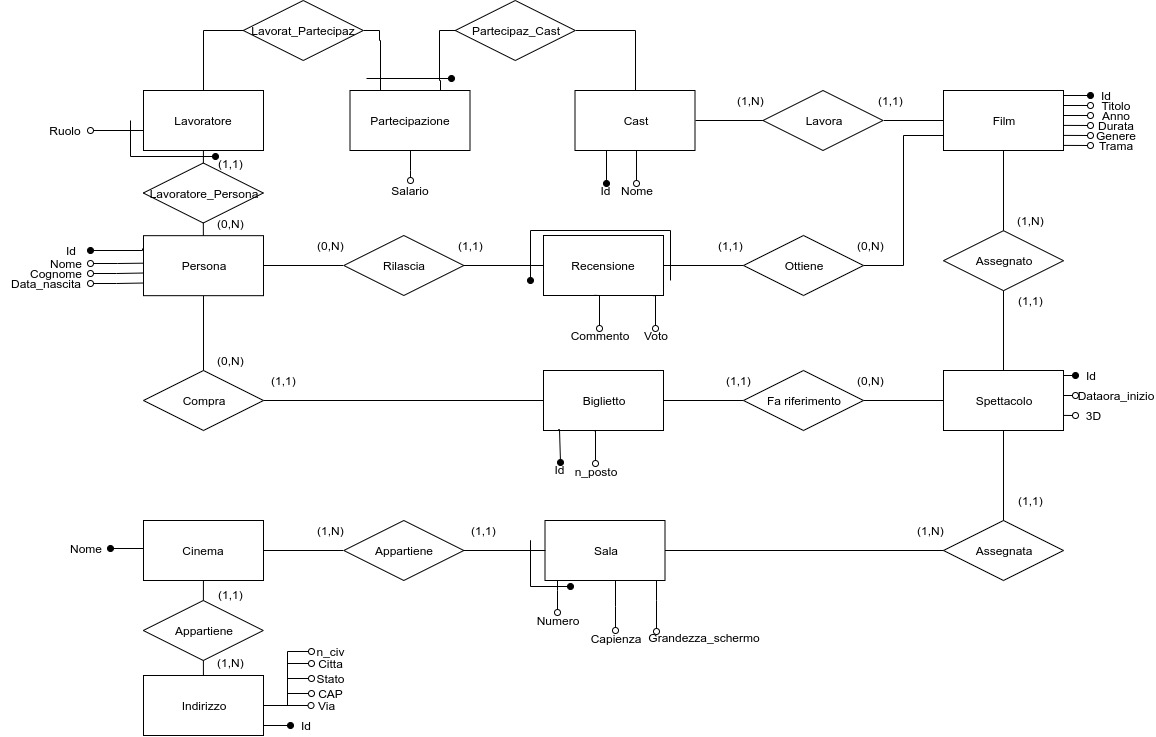
\includegraphics[width=\textwidth, height=13cm]{Schemas/SchemaER_Rev}
	\subsection{Traduzione nel modello relazionale}
	\textbf{Cinema}(\underline{Nome}, Id\_Indirizzo)\\
	\textit{vincolo di integrita' referenziale tra "Id\_Indirizzo" ed "Id" in Indirizzo.}\\\\
	\textbf{Sala}(\underline{Numero}, \underline{Nome\_Cinema}, Capienza, Grandezza\_schermo)\\
	\textit{Vincolo di integrita' referenziale tra "Nome\_Cinema" e "Nome" in Cinema.}\\\\
	\textbf{Spettacolo}(\underline{Id}, Dataora\_inizio, 3D, Id\_Film, Num\_Sala, Nome\_Cinema)\\
	\textit{Vincolo di integrita' referenziale tra "Id\_Film" ed "Id" in Film, "Num\_Sala" e "Numero" in Sala e tra "Nome\_Cinema" e "Cinema" in Sala.}\\\\
	\textbf{Biglietto}(\underline{Id\_Spettacolo}, \underline{Id\_Persona}, n\_posto)\\
	\textit{Vincolo di integrita' referenziale tra "Id\_Spettacolo" ed "Id" in Spettacolo e tra "Id\_Persona" e "Id" in Persona.}\\\\
	\textbf{Film}(\underline{Id}, Titolo, Anno, Durata, Genere, Trama, Id\_Cast)\\
	\textit{Vincolo di integrita' referenziale tra "Id\_Cast" e "Id" in Cast}.\\\\
	\textbf{Recensione}(\underline{Id\_Film}, \underline{Id\_Persona}, Commento, Voto)\\
	\textit{Vincolo di integrita' referenziale tra "Id\_Film" e "Id" in Film e tra "Id\_Persona" e "Id" in Persona.}\\\\
	\textbf{Persona}(\underline{Id}, Nome, Cognome, Data\_nascita)\\\\
	\textbf{Lavoratore}(\underline{Id\_Persona}, \underline{Id\_Cast}, \underline{Ruolo}, Salario)\\	
	\textit{Vincolo di integrita' referenziale tra "Id\_Persona" e "Id" in Persona e tra "Id\_Cast" e "Id" in Cast}.\\\\
	\textbf{Cast}(\underline{Id}, Nome).\\\\
	\textbf{Indirizzo}(\underline{Id}, Via, Citta, n\_civ, Stato, Cap)\\\\
	\section{Query e Indici}
	\subsection{Query}
	\paragraph{Query1}
	Numero di recensioni di persone che non hanno visto il film, quindi di conseguenza non valide.		
	\begin{lstlisting}[language=SQL]
	SELECT p.Id, p.Nome, p.Cognome, COUNT(r.Id_Persona) AS 'N. Recensioni non valide'
	FROM Recensione r JOIN Persona p ON (r.Id_Persona=p.Id) LEFT JOIN (SELECT DISTINCT f.Id AS Id_Film, b.Id_Persona AS Id_Persona, f.Titolo as Titolo
	FROM Biglietto b, Spettacolo s, Film f
	WHERE  s.Id=b.Id_Spettacolo AND f.Id=s.Id_Film
	) sq ON (r.Id_Persona= sq.Id_persona AND r.Id_Film=sq.Id_Film)
	WHERE sq.Id_Persona IS NULL
	GROUP BY p.Id	
	--Risultato Query
	+----+----------+-----------+--------------------------+
	| Id | Nome     | Cognome   | N. Recensioni non valide |
	+----+----------+-----------+--------------------------+
	|  1 | Mario    | Rossi     |                        4 |
	|  2 | Matteo   | Verdi     |                        6 |
	|  3 | Stefano  | Minto     |                        6 |
	| .. |     .... |     ...   |                       ...|
	+----+----------+-----------+--------------------------+	
	\end{lstlisting}
	\pagebreak
	\paragraph{Query2}
	Voto medio per film in base alle recensioni valide.
	\begin{lstlisting}[language=SQL]
	SELECT sq.Titolo, AVG(r.Voto) AS 'Voto Medio'
	FROM Recensione r JOIN (SELECT DISTINCT f.Id AS Id_Film, b.Id_Persona AS Id_Persona, f.Titolo as Titolo
	FROM Biglietto b, Spettacolo s, Film f
	WHERE  s.Id=b.Id_Spettacolo AND f.Id=s.Id_Film
	) sq ON (r.Id_Persona= sq.Id_persona AND r.Id_Film=sq.Id_Film)
	GROUP BY sq.Titolo	
	--Risultato Query
	+-------------------+------------+
	| Titolo            | Voto Medio |
	+-------------------+------------+
	| Cinepanettone     |     3.5000 |
	| Jumanji           |     1.6667 |
	| Mediterraneo      |     4.0000 |
	|                ...|        ... |
	+-------------------+------------+	
	\end{lstlisting}
	\paragraph{Query3}
	Affluenza di persone per cinema.
	\begin{lstlisting}[language=SQL]
	SELECT s.Nome_Cinema AS Cinema, COUNT(b.Id_Persona) AS Affluenza
	FROM Biglietto b JOIN Spettacolo s ON (b.Id_Spettacolo=s.Id)
	GROUP BY s.Nome_Cinema
	ORDER by s.Nome_Cinema	
	--Risultato Query
	+-------------+-----------+
	| Cinema      | Affluenza |
	+-------------+-----------+
	| D4C Marcon  |        10 |
	| D4C Mestre  |         4 |
	| D4C Milano  |         4 |
	|          ...|       ... |
	+-------------+-----------+	
	\end{lstlisting}
	\paragraph{Query4}
	Lista attore/sceneggiatore/produttore/regista piu' pagato.
	\begin{lstlisting}[language=SQL]
	SELECT sq.Id_Persona AS ID, p.Nome, p.Cognome, p.Sesso, sq.Ruolo, MAX(sq.Salario) AS Salario
	FROM (SELECT Id_Persona, Ruolo, SUM(Salario) AS Salario
	FROM Lavoratore l
	GROUP BY Id_Persona, Ruolo) AS sq JOIN Persona p ON (p.Id=sq.Id_Persona)
	GROUP BY sq.Ruolo	
	--Risultato Query
	+----+-----------+----------+-------+---------------+---------+
	| ID | Nome      | Cognome  | Sesso | Ruolo         | Salario |
	+----+-----------+----------+-------+---------------+---------+
	|  1 | Mario     | Rossi    | M     | Attore        |   25000 |
	|  4 | Alessando | Rebeschi | M     | Regista       |   30000 |
	|  8 | Enrico    | Marcato  | M     | Produttore    |   50000 |
	|  4 | Alessando | Rebeschi | M     | Sceneggiatore |   15000 |
	+----+-----------+----------+-------+---------------+---------+
	
	\end{lstlisting}
	\paragraph{Query5}
	
	Lista film a cui ha partecipato uno specifico attore. \\\textit{In questo caso viene preso come esempio la persona con Id=21.}
	\begin{lstlisting}[language=SQL]
	SELECT f.Titolo, f.Anno, f.Durata, f.Genere
	FROM Film f JOIN `Cast` c ON c.Id=f.Id_Cast JOIN Lavoratore l ON l.Id_Cast=c.Id
	WHERE l.Ruolo='Attore' AND l.Id_Persona=21	
	--Risultato Query
	+-------------------+------+----------+----------+
	| Titolo            | Anno | Durata   | Genere   |
	+-------------------+------+----------+----------+
	| Film Indie        | 2014 | 00:50:00 | Thriller |
	| Storie Spaventose | 2010 | 00:50:00 | Horror   |
	+-------------------+------+----------+----------+
	
	\end{lstlisting}
	\paragraph{Query6}
	Lista rapporto incasso a spettacolo
	\begin{lstlisting}[language=SQL]
	SELECT s.Id AS Spettacolo, s.Nome_Cinema AS Cinema, f.Titolo AS Titolo, COUNT(b.Id_Persona) AS Affluenza, COUNT(b.Id_Persona)*10 as Incasso
	FROM Spettacolo s LEFT JOIN Biglietto b ON b.Id_Spettacolo=s.Id JOIN Film f ON f.Id=s.Id_Film
	GROUP BY s.Id
	ORDER BY Affluenza DESC
	--Risultato Query
	+------------+-------------+-------------------+-----------+---------+
	| Spettacolo | Cinema      | Titolo            | Affluenza | Incasso |
	+------------+-------------+-------------------+-----------+---------+
	|         11 | D4C Marcon  | The Matrix        |         7 |      70 |
	|         21 | D4C Silea   | The Matrix        |         3 |      30 |
	|          1 | D4C Mestre  | The Matrix        |         2 |      20 |
	|         41 | D4C Treviso | The Matrix        |         2 |      20 |
	|        ... |          ...|                ...|       ... |     ... |
	+------------+-------------+-------------------+-----------+---------+	
	
	\end{lstlisting}
	\subsection{Indici}
	\subsubsection{Studio caso d'uso}
	Ipotizzando di avere il database con un'ampia quantita' di dati, si ipotizza che:
	\begin{itemize}
		\item La tabella \textbf{Spettacolo} contanga molte tuple
		\item Nella tabella \textbf{Spettacolo} vengono aggiunti molto frequentemente nuove tuple
		\item La stessa viene consultata spesso per l'orario inizio spettacoli
		\item La tabella \textbf{Film} contenga molte tuple
		\item Nella tabella \textbf{Film} non poche volte al mese vengano aggiunti nuovi film
		\item La stessa viene consultata spesso per il titolo del film
		\item La tabella \textbf{Persona} contanga molte tuple
		\item Nella tabella \textbf{Persona} vengono aggiunti spesso nuove tuple
		\item La stessa viene colsultata spesso per la ricerca di un film tramite attore, ricercandolo per cognome
	\end{itemize}
	\subsubsection{Riconoscimento tabelle da indicizzare}
	\begin{itemize}
		\item \textbf{Spettacolo}
		\item \textbf{Film}
		\item \textbf{Persona}
	\end{itemize}
	\subsubsection{Implementazione dell'indice}
	\begin{lstlisting}[language=SQL]
	CREATE INDEX idx_OrarioSpettacoli ON Spettacolo (Dataora_inizio);
	CREATE INDEX idx_TitoloFilm ON Film (Titolo);
	CREATE INDEX idx_CognomePersona ON Persona (Cognome);
	
	\end{lstlisting}
\end{document}
